\chapter{Mesh Generation}\label{cha:Mesh-Generation}

The first step in running a spectral-element simulation consists of
constructing a high-quality mesh for the region under consideration.
We provide two possibilities to do so: (1) relying on the external,
hexahedral mesher CUBIT, or (2) using the provided, internal mesher
\texttt{xmeshfem3D}. In the following, we explain these two approaches.


\section{Meshing with \texttt{CUBIT}}\label{cha:Running-the-Mesher-CUBIT}

CUBIT is a meshing tool suite for the creation of finite-element meshes
for arbitrarily shaped models. It has been developed and maintained
at Sandia National Laboratories and can be purchased for a small academic
institutional fee at \url{http://cubit.sandia.gov}. Our experience
showed that using CUBIT greatly facilitates and speeds up the generation
and preparation of hexahedral, conforming meshes for a variety of
geophysical models with increasing complexity.

\begin{figure}[htbp]
\begin{centering}
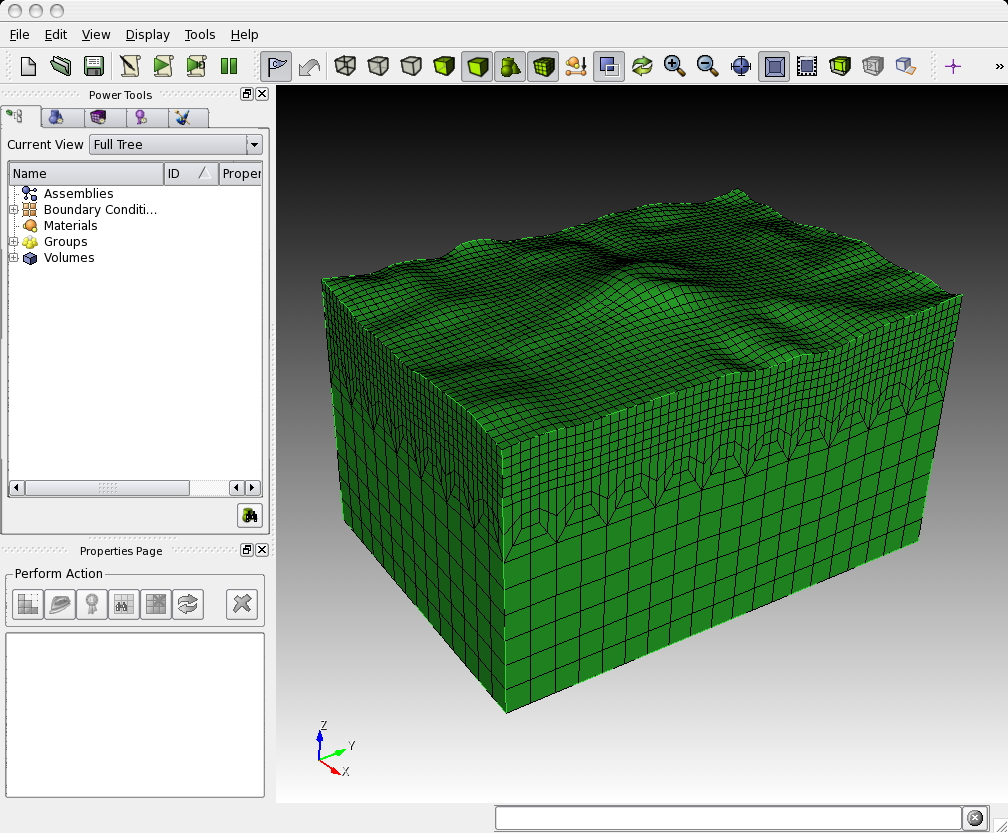
\includegraphics[width=0.6\textwidth]{figures/mount-cubit.jpg}
\par
\end{centering}
\caption{Example of the graphical user interface of CUBIT. The hexahedral mesh
shown in the main display consists of a hexahedral discretization
of a single volume with topography.}
\label{fig:mount.cubit}
\end{figure}

\noindent
The basic steps in creating a load-balanced, partitioned mesh with
CUBIT are:
\begin{description}
\item [{1.}] setting up a hexahedral mesh with CUBIT,
\item [{2.}] exporting the CUBIT mesh into a SPECFEM3D Cartesian file format
and
\item [{3.}] partitioning the SPECFEM3D Cartesian mesh files for a chosen
number of cores.
\end{description}
Examples are provided in the SPECFEM3D Cartesian package in the subdirectory
\texttt{EXAMPLES/}. We strongly encourage you to contribute your own
example to this package by contacting the CIG Computational Seismology
Mailing List \urlwithparentheses{cig-seismo@geodynamics.org}.


\subsection{Creating the Mesh with CUBIT}

For the installation and handling of the CUBIT meshing tool suite,
please refer to the CUBIT user manual and documentation. In order
to give you a basic understanding of how to use CUBIT for our purposes,
examples are provided in the SPECFEM3D Cartesian package in the subdirectory
\texttt{EXAMPLES/}:
\begin{description}
\item [{\texttt{homogeneous\_halfspace}}] Creates a single block model
and assigns elastic material parameters.
\item [{\texttt{layered\_halfspace}}] Combines two different, elastic material
volumes and creates a refinement layer between the two. This example
can be compared for validation against the solutions provided in subdirectory
~\\
 \texttt{VALIDATION\_3D\_SEM\_SIMPLER\_LAYER\_SOURCE\_DEPTH/}.
\item [{\texttt{waterlayered\_halfspace}}] Combines an acoustic and elastic
material volume as in a schematic marine survey example.
\item [{\texttt{tomographic\_model}}] Creates a single block model whose
material properties will have to be read in from a tomographic model
file during the databases creation by \texttt{xgenerate\_databases}.
\end{description}
%
\begin{figure}[htbp]
\begin{centering}
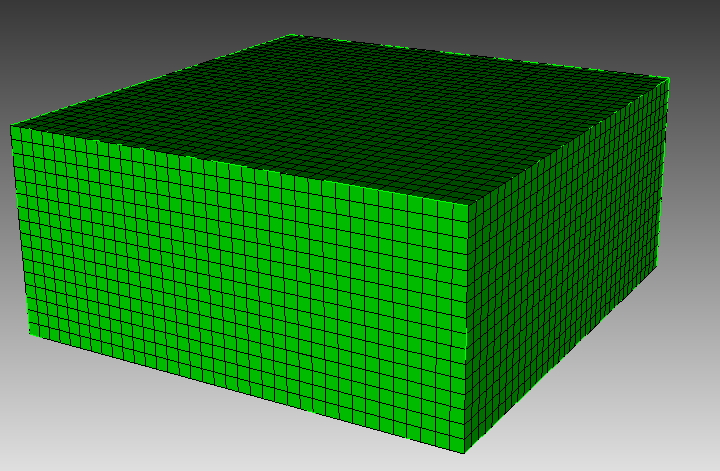
\includegraphics[width=0.45\textwidth]{figures/example-homogeneous.jpg}
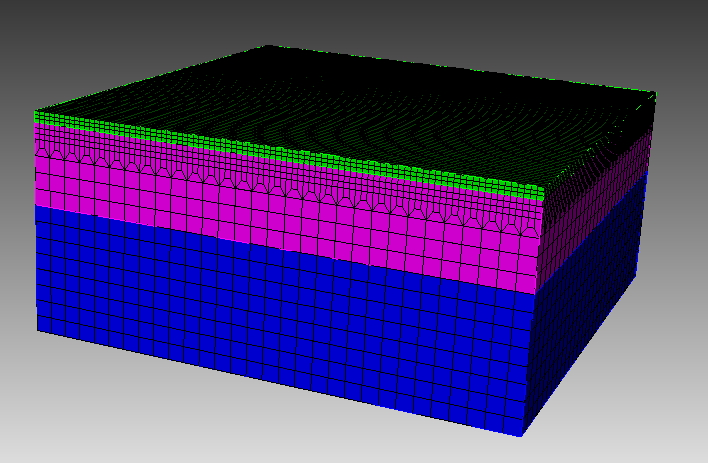
\includegraphics[width=0.45\textwidth]{figures/example-2layers.jpg} \\
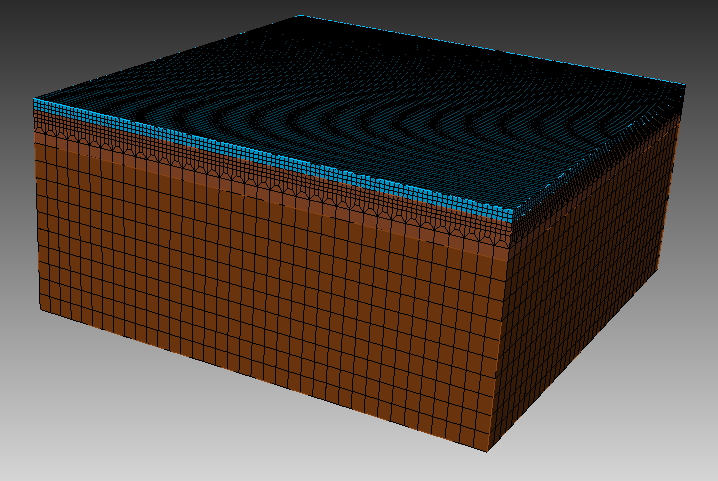
\includegraphics[width=0.45\textwidth]{figures/example-water.jpg}
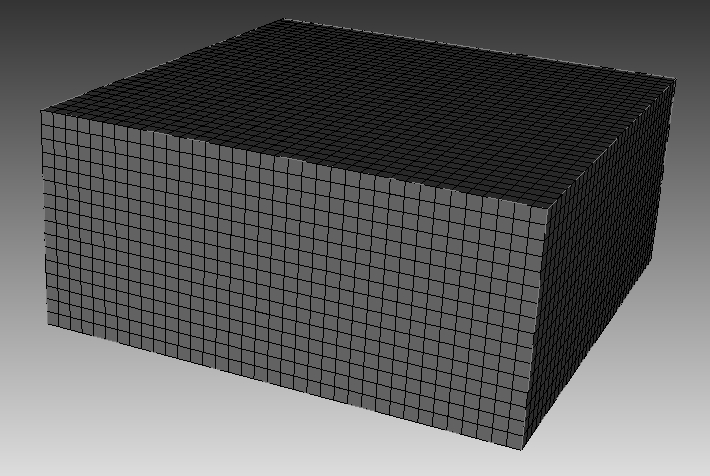
\includegraphics[width=0.45\textwidth]{figures/example-tomo.jpg}
\par
\end{centering}
\caption{Screenshots of the CUBIT examples provided in subdirectory \texttt{EXAMPLES/}:
homogeneous halfspace (top-left), layered halfspace (top-right), water
layered halfspace (bottom-left) and tomographic model (bottom-right).}
\label{fig:examples.cubit}
\end{figure}


In each example subdirectory you will find a \texttt{README} file,
which explains in a step-by-step tutorial the workflow for the example.
Please feel free to contribute your own example to this package by
contacting the CIG Computational Seismology Mailing List \urlwithparentheses{cig-seismo@geodynamics.org}.\\

In some cases, to re-create the meshes for the examples given, just type
\begin{verbatim}
claro ./create_mesh.py
\end{verbatim}
or similar from the command line (\texttt{claro} is the command to run CUBIT from the command line).

{\it IMPORTANT:} In order to correctly set up GEOCUBIT and run the examples, please read the file called \texttt{EXAMPLES/README};
in particular, please make sure you correctly set up the Python paths as indicated in that file.

Concerning the script \texttt{create\_mesh.py}, you may find the option \texttt{use\_explicit} which chooses how to assign the material properties for the volume (or domain):
\begin{itemize}
\item[(1)] one way is to explicitly assign block attributes to the block of the corresponding volume, by commands like:
\begin{verbatim}
cubit.cmd('block '+str(id_block)+' attribute index 2 2800') # vp
\end{verbatim}
This is done when using \texttt{use\_explicit = 1} in the script. The final command:
\begin{verbatim}
cubit2specfem3d.export2SPECFEM3D('MESH/')
\end{verbatim}
will then create the corresponding \texttt{MESH/nummaterial\_velocity\_file} for all such defined block volumes/domains.

\item[(2)] the other option with \texttt{use\_explicit = 0} is to let GEOCUBIT deal with a dummy entry and then overwrite the \texttt{nummaterial\_velocity\_file} at the end with a corresponding command section:
\begin{verbatim}
f = open(nummaterial_velocity_file,'w')
\end{verbatim}
This second way is chosen by default because GEOCUBIT can handle partitions for several processes and glues everything together automatically. Thus, it adds some more sophistication when the model gets more complicated than just this single volume example.
\end{itemize}
You will find out by experimenting what is easier for your case.


\subsection{Exporting the Mesh with \texttt{run\_cubit2specfem3d.py} }\label{subsec:Exporting-the-Mesh}

Once the geometric model volumes in CUBIT are meshed, you prepare
the model for exportation with the definition of material blocks and
boundary surfaces. Thus, prior to exporting the mesh, you need to
define blocks specifying the materials and absorbing boundaries in
CUBIT. This process could be done automatically using the script \texttt{run\_cubit2specfem3d.py}
if the mesh meets some conditions or manually, following the block
convention:
\begin{description}
\item [{material\_name}] Each material should have a specific block defined
by a unique name. The name convention of the material is to start
with either \textbf{'elastic'} or \textbf{'acoustic'}. It must be then followed by a
unique identifier, e.g. \textbf{'elastic 1'}, \textbf{'elastic 2'}, etc. The additional
attributes to the block define the material description.


For an elastic material:
\begin{description}
\item [{material\_id}] An integer value which is unique for this material.
\item [{Vp}] P-wave speed of the material (given in m/s).
\item [{Vs}] S-wave speed of the material (given in m/s).
\item [{rho}] density of the material (given in kg/m$^{3}$).
\item [{Q}] quality factor to use in case of a simulation with attenuation
turned on. It should be between 1 and 9000. In case no attenuation
information is available, it can be set to zero. You can either specify a single Q value,
in which case it will be assumed to be pure shear attenuation $Q_{\mu}$, or two
separate values for bulk and shear attenuation, $Q_{\kappa}$ and $Q_{\mu}$ respectively.
Note that Qmu is always equal to Qs, but Qkappa is in general not equal to Qp. To convert one to the other see doc/note\_on\_Qkappa\_versus\_Qp.pdf and utils/attenuation/conversion\_from\_Qkappa\_Qmu\_to\_Qp\_Qs\_from\_Dahlen\_Tromp\_959\_960.f90.

Please note that your Vp- and Vs-speeds are given for a reference frequency. To change
this reference frequency, you change the value of \texttt{ATTENUATION\_f0\_REFERENCE}
in the main constants file \texttt{constants.h} found in subdirectory
\texttt{src/shared/}.
The code uses a constant $Q$ quality factor, write(IMAIN,*) "but approximated based on a series of Zener standard linear solids (SLS).
The approximation is thus performed in a given frequency band determined based on that \texttt{ATTENUATION\_f0\_REFERENCE} reference frequency.
\item [{anisotropic\_flag}] Flag describing the anisotropic model to use
in case an anisotropic simulation should be conducted. See the file
\texttt{model\_aniso.f90} in subdirectory \texttt{src/generate\_databases/}
for an implementation of the anisotropic models. In case no anisotropy
is available, it can be set to zero.
\end{description}

Note that this material block has to be defined using all the volumes
which belong to this elastic material. For volumes belonging to another,
different material, you will need to define a new material block.


For an acoustic material:
\begin{description}
\item [{material\_id}] An integer value which is unique for this material.
\item [{Vp}] P-wave speed of the material (given in m/s).
\item [{0}] S-wave speed of the material is ignored.
\item [{rho}] density of the material (given in kg/m$^{3}$).
\end{description}
\item [{face\_topo}] Block definition for the surface which defines the
free surface (which can have topography). The name of this block must
be 'face\_topo', the block has to be defined using all the surfaces
which constitute the complete free surface of the model.
\item [{face\_abs\_xmin}] Block definition for the faces on the absorbing
boundaries, one block for each surface with x=Xmin.
\item [{face\_abs\_xmax}] Block definition for the faces on the absorbing
boundaries, one block for each surface with x=Xmax.
\item [{face\_abs\_ymin}] Block definition for the faces on the absorbing
boundaries, one block for each surface with y=Ymin.
\item [{face\_abs\_ymax}] Block definition for the faces on the absorbing
boundaries, one block for each surface with y=Ymax.
\item [{face\_abs\_bottom}] Block definition for the faces on the absorbing
boundaries, one block for each surface with z=bottom.
\end{description}
%
\begin{figure}[htbp]
\begin{centering}
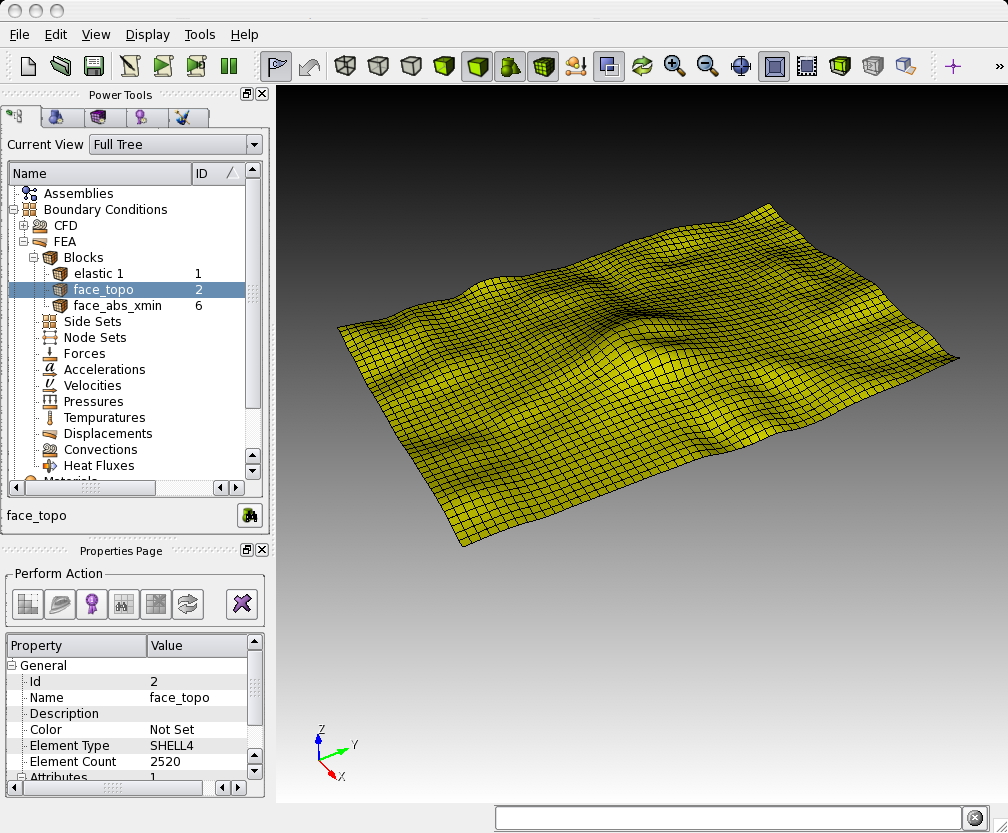
\includegraphics[width=0.45\textwidth]{figures/mount-surface.jpg}
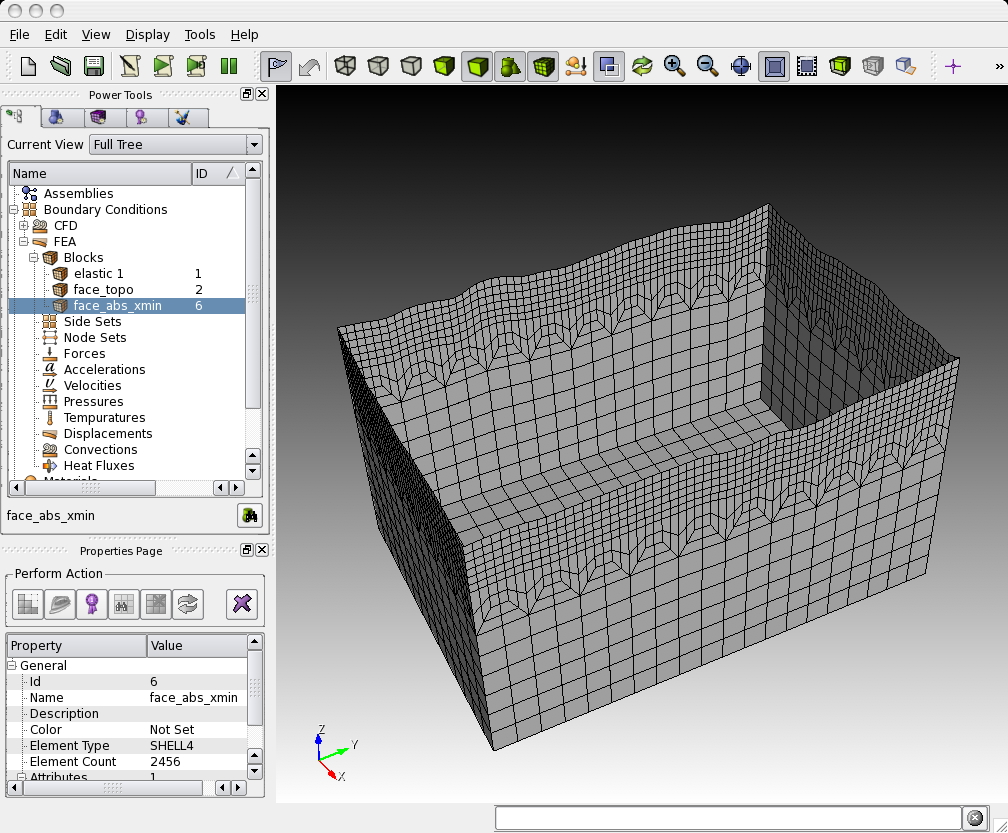
\includegraphics[width=0.45\textwidth]{figures/mount-abs.jpg}
\par
\end{centering}
\caption{Example of the block definitions for the free surface 'face\_topo'
(left) and the absorbing boundaries, defined in a single block 'face\_abs\_xmin'
(right) in CUBIT.}
\label{fig:mount.abs}
\end{figure}


Optionally, instead of specifying for each surface at the boundaries
a single block like mentioned above, you can also specify a single
block for all boundary surfaces and name it as one of the absorbing
blocks above, e.g. 'face\_abs\_xmin'.

After the block definitions are done, you export the mesh using the
script \texttt{cubit2specfem3d.py} provided in each of the example
directories (linked to the common script \texttt{CUBIT\_GEOCUBIT/cubit2specfem3d.py}).
If the export was successful, you should find the following
files in a subdirectory \texttt{MESH/}:
\begin{description}
\item [{absorbing\_cpml\_file}] \textbf{(only needed in case of C-PML absorbing
conditions)} Contains on the first line the total number of C-PML
spectral elements in the mesh, and then on the following line the
list of all these C-PML elements with two numbers per line: first
the spectral element number, and then a C-PML flag indicating to which
C-PML layer(s) that element belongs, according to the following convention:

\begin{itemize}
\item Flag = 1 : element belongs to a X CPML layer only (either in Xmin or in Xmax),
\item Flag = 2 : element belongs to a Y CPML layer only (either in Ymin or in Ymax),
\item Flag = 3 : element belongs to a Z CPML layer only (either in Zmin or in Zmax),
\item Flag = 4 : element belongs to a X CPML layer and also to a Y CPML layer,
\item Flag = 5 : element belongs to a X CPML layer and also to a Z CPML layer,
\item Flag = 6 : element belongs to a Y CPML layer and also to a Z CPML layer,
\item Flag = 7 : element belongs to a X, to a Y and to a Z CPML layer, i.e., it belongs to a CPML corner.
\end{itemize}

Note that it does not matter whether an element belongs to a Xmin
or to a Xmax CPML, the flag is the same in both cases; the same is
true for Ymin and Ymax, and also Zmin and Zmax.


When you have an existing CUBIT (or similar) mesh stored in SPECFEM3D
format, i.e., if you have existing \texttt{nodes\_coords\_file}
and \texttt{mesh\_file} files but do not know
how to assign CPML flags to them, we have created a small serial Fortran
program that will do that automatically for you, i.e., which will
create the \texttt{absorbing\_cpml\_file} for
you. That program is: \\
\texttt{utils/CPML/convert\_external\_layers\_of\_a\_given\_mesh\_to\_CPML\_layers.f90},\\
and a small Makefile is provided in that directory (utils/CPML).


IMPORTANT: it is your responsibility to make sure that in the input
CUBIT (or similar) mesh that this code will read in SPECFEM3D format
from files \texttt{nodes\_coords\_file} and \texttt{mesh\_file}
you have created layers of elements that constitute a layer of constant
thickness aligned with the coordinate grid axes (X, Y and/or Z), so
that this code can assign CPML flags to them. This code does NOT check
that (because it cannot, in any easy way). The mesh inside these CPML
layers does not need to be structured nor regular, any non-structured
mesh is fine as long as it has flat PML inner and outer faces, parallel
to the axes, and thus of a constant thickness. The thickness can be
different for the X, Y and Z sides. But for X it must not vary, for
Y it must not vary, and for Z it must not vary. If you do not know
the exact thickness, you can use a slightly LARGER value in this code
(say 2\% to 5\% more) and this code will fix that and will adjust
it; never use a SMALLER value otherwise this code will miss some CPML
elements.


Note: in a future release we will remove the constraint of having
CPML layers aligned with the coordinate axes; we will allow for meshes
that are titled by any constant angle in the horizontal plane. However
this is not implemented yet.


Note: in the case of fluid-solid layers in contact, the fluid-solid
interface currently needs to be flat and horizontal inside the CPML
layer (i.e., bathymetry should become flat and horizontal when entering
the CPML); this (small) constraint will probably remain in the code
for a while because it makes fluid-solid matching inside the CPML
much easier.

\item [{materials\_file}] Contains the material associations for each element.
The format is:
\begin{verbatim}
element_ID material_ID
\end{verbatim}

where \texttt{element\_ID} is the element identifier and \texttt{material\_ID}
is a unique identifier, positive (for materials taken from this list
of materials, i.e. for which each spectral element has constant material
properties taken from this list) or negative (for tomographic models,
i.e. for spectral element whose real velocities and density will be
assigned later by calling an external function to define model variations,
for instance in the case of tomographic models; in such a case, material
properties can vary inside each spectral element, i.e. be different
at each of its Gauss-Lobatto-Legendre grid points).

\item [{nummaterial\_velocity\_file}] Defines the material properties.

\begin{itemize}
\item For classical materials (i.e., spectral elements for which the velocity
and density model will not be assigned by calling an external function
to define for instance a tomographic model), the format is:

\begin{verbatim}
domain_ID material_ID rho vp vs Qkappa Qmu anisotropy_flag
\end{verbatim}

where \texttt{\textbf{domain\_ID}}\textbf{ is 1 for acoustic and 2
for elastic or viscoelastic materials,} \texttt{material\_ID} a unique
identifier, \texttt{rho} the density in $kg\, m^{-3}$, \texttt{vp}
the P-wave speed in $m\, s^{-1}$, \texttt{vs} the S-wave speed in
$m\, s^{-1}$, \texttt{Q} the quality factor and \texttt{anisotropy\_flag}
an identifier for anisotropic models.
Note that both \texttt{Qkappa} and \texttt{Qmu} are ignored
by the code unless \texttt{ATTENUATION} is set. If you want a model
with no \texttt{Qmu} attenuation, both set \texttt{ATTENUATION} to
\texttt{.false.} in the \texttt{Par\_file} and set \texttt{Qmu} to
9999 here. If you want a model with no \texttt{Qkappa} attenuation, set \texttt{Qkappa} to 9999 here.
Note that Qmu is always equal to Qs, but Qkappa is in general not equal to Qp. To convert one to the other see doc/note\_on\_Qkappa\_versus\_Qp.pdf and utils/attenuation/conversion\_from\_Qkappa\_Qmu\_to\_Qp\_Qs\_from\_Dahlen\_Tromp\_959\_960.f90.

\item For tomographic velocity models, please read Chapter \ref{cha:-Changing-the}
and Section \ref{sec:Using-tomographic} `Using external tomographic
Earth models' for further details.
\end{itemize}
\item [{nodes\_coords\_file}] Contains the point locations in Cartesian
coordinates of the mesh element corners.
\item [{mesh\_file}] Contains the mesh element connectivity. The hexahedral
elements can have 8 or 27 nodes.\\
 See picture doc/mesh\_numbering\_convention/numbering\_convention\_27\_nodes.jpg
to see\\
 in which (standard) order the points must be cited. In the case of
8 nodes, just include the first 8 points.
\item [{free\_or\_absorbing\_surface\_file\_zmax}] Contains the free surface
connectivity or \\
 the surface connectivity of the absorbing boundary surface at the
top (Zmax), \\
 depending on whether the top surface is defined as free or absorbing
(\texttt{STACEY\_INSTEAD\_OF\_FREE\_SURFACE} in \texttt{DATA/Par\_file}). \\
 You should put both the surface of acoustic regions and of elastic
regions in that file; that is, list all the element faces that constitute
the surface of the model in that file.
\item [{absorbing\_surface\_file\_xmax}] Contains the surface connectivity
of the absorbing boundary surface at Xmax \\
(also needed in the case of C-PML absorbing conditions, in order for
the code to be able to impose Dirichlet conditions on their outer
edge).
\item [{absorbing\_surface\_file\_xmin}] Contains the surface connectivity
of the absorbing boundary surface at Xmin \\
(also needed in the case of C-PML absorbing conditions, in order for
the code to be able to impose Dirichlet conditions on their outer
edge).
\item [{absorbing\_surface\_file\_ymax}] Contains the surface connectivity
of the absorbing boundary surface at Ymax \\
(also needed in the case of C-PML absorbing conditions, in order for
the code to be able to impose Dirichlet conditions on their outer
edge).
\item [{absorbing\_surface\_file\_ymin}] Contains the surface connectivity
of the absorbing boundary surface at Ymin \\
(also needed in the case of C-PML absorbing conditions, in order for
the code to be able to impose Dirichlet conditions on their outer
edge).
\item [{absorbing\_surface\_file\_bottom}] Contains the surface connectivity
of the absorbing boundary surface at the bottom (Zmin) \\
(also needed in the case of C-PML absorbing conditions, in order for
the code to be able to impose Dirichlet conditions on their outer
edge).
\end{description}
These mesh files are needed as input files for the partitioner \texttt{xdecompose\_mesh}
to load-balance the mesh. Please see the next section for further
details.

In directory "CUBIT\_GEOCUBIT/" we provide a script that can help doing the above tasks of exporting a CUBIT mesh
to SPECFEM3D format automatically for you: "run\_cubit2specfem3d.py".
Just edit them to indicate the path to your local installation of CUBIT and also the name of the *.cub existing CUBIT mesh file
that you want to export to SPECFEM3D format. These scripts will do the conversion for you automatically except assigning material properties
to the different mesh layers. To do so, you will then need to edit the file
called "nummaterial\_velocity\_file" that will have just been created and change it from the prototype created:

{\footnotesize
\begin{verbatim}
0 1 vol1 --> syntax: #material_domain_id #material_id #rho #vp #vs #Q_kappa #Q_mu #anisotropy
0 2 vol2 --> syntax: #material_domain_id #material_id #rho #vp #vs #Q_kappa #Q_mu #anisotropy
\end{verbatim}
}
\noindent
(where "vol1" and "vol2" here represent the volume labels that you have set while creating the mesh in CUBIT)
to for instance

{\footnotesize
\begin{verbatim}
2 1 1500 2300 1800 9999.0 9999.0 0
2 2 1600 2500 20000 9999.0 9999.0 0
\end{verbatim}
}

\subsubsection*{Checking the mesh quality}

The quality of the mesh may be inspected more precisely based upon
the serial code in the file \texttt{check\_mesh\_quality\_}~\\
 \texttt{CUBIT\_Abaqus.f90} located in the directory \texttt{src/check\_mesh\_quality\_CUBIT\_Abaqus/}.
Running this code is optional because no information needed by the
solver is generated.

Prior to running and compiling this code, you have to export your
mesh in CUBIT to an ABAQUS (.inp) format. For example, export mesh
block IDs belonging to volumes in order to check the quality of the
hexahedral elements. You also have to determine a number of parameters
of your mesh, such as the number of nodes and number of elements and
modify the header of the \texttt{check\_mesh\_quality\_CUBIT\_Abaqus.f90}
source file in directory \texttt{src/check\_mesh\_quality\_CUBIT\_Abaqus/}.

\noindent
Then, in the main directory, type
{\small
\begin{verbatim}
make xcheck_mesh_quality
\end{verbatim}
}
and use
{\small
\begin{verbatim}
./bin/xcheck_mesh_quality
\end{verbatim}
}
to generate an %not supported: AVS output file (\texttt{\small AVS\_meshquality.inp} in AVS UCD format) or
OpenDX output file (\texttt{\small DX\_mesh\_quality.dx}{\small )
that can be used to investigate mesh quality, e.g. skewness of elements,
and a Gnuplot histogram (}\texttt{\small mesh\_quality\_histogram.txt}{\small )
that can be plotted with gnuplot (type `}\texttt{\small gnuplot plot\_mesh\_quality\_histogram.gnu}{\small ').
The histogram is also printed to the screen. Analyze that skewness
histogram of mesh elements to make sure no element has a skewness
above approximately 0.75, otherwise the mesh is of poor quality (and
if even a single element has a skewness value above 0.80, then you
must definitely improve the mesh). If you want to start designing
your own meshes, this tool is useful for viewing your creations. You
are striving for meshes with elements with `cube-like' dimensions,
e.g., the mesh should contain no very elongated or skewed elements.}{\small \par}


\subsection{Partitioning the Mesh with \texttt{xdecompose\_mesh}}

The SPECFEM3D Cartesian software package performs large scale simulations
in a parallel 'Single Process Multiple Data' way. The spectral-element
mesh created with CUBIT needs to be distributed on the processors.
This partitioning is executed once and for all prior to the execution
of the solver so it is referred to as a static mapping.

An efficient partitioning is important because it leverages the overall
running time of the application. It amounts to balance the number
of elements in each slice while minimizing the communication costs
resulting from the placement of adjacent elements on different processors.
\texttt{decompose\_mesh} depends on the SCOTCH library \citep{PeRo96},
which provides efficient static mapping, graph and mesh partitioning
routines. SCOTCH is a free software package developed by Fran\c{c}ois
Pellegrini et al. from LaBRI and INRIA in Bordeaux, France, downloadable
from the web page \url{https://gforge.inria.fr/projects/scotch/}.\\


In most cases, the configuration with \texttt{./configure~FC=ifort}
should be sufficient. During the configuration process, the script
tries to find existing SCOTCH installations. In case your system has
no pre-existing SCOTCH installation, we provide the source code of
SCOTCH, which is released open source under the French CeCILL-C version
1 license, in directory \texttt{src/decompose\_mesh/scotch\_5.1.12b}.
This version gets bundled with the compilation of the SPECFEM3D Cartesian
package if no libraries could have been found. If this automatic compilation
of the SCOTCH libraries fails, please refer to file INSTALL.txt in
that directory to see further details how to compile it on your system.
In case you want to use a pre-existing installation, make sure you
have correctly specified the path of the SCOTCH library when using
the option \texttt{-{}-with-scotch-dir} with the \texttt{./configure}
script. In the future you should be able to find more recent versions
at \url{http://www.labri.fr/perso/pelegrin/scotch/scotch_en.html}.\\


\begin{figure}[htbp]
\begin{centering}
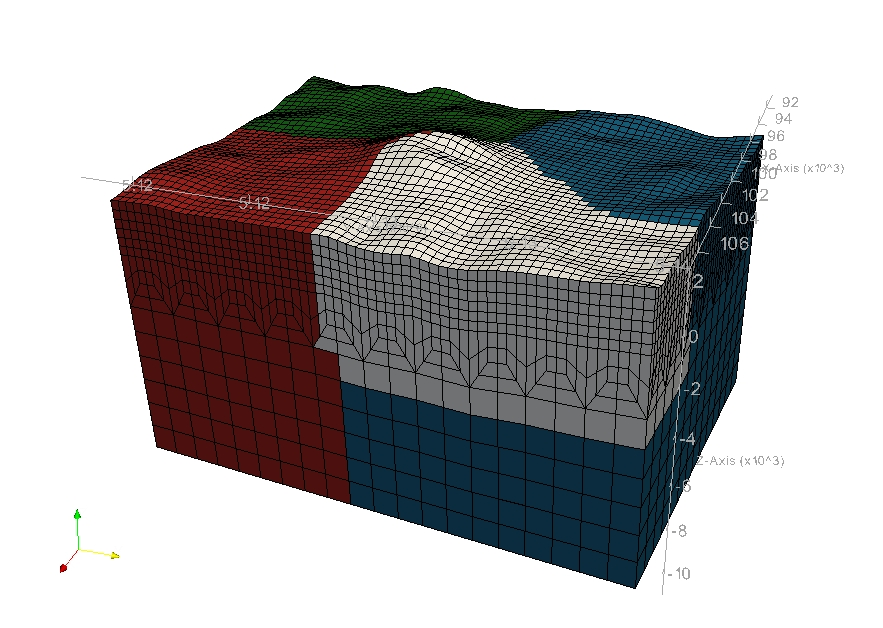
\includegraphics[width=0.45\textwidth]{figures/mount-partitions.jpg}
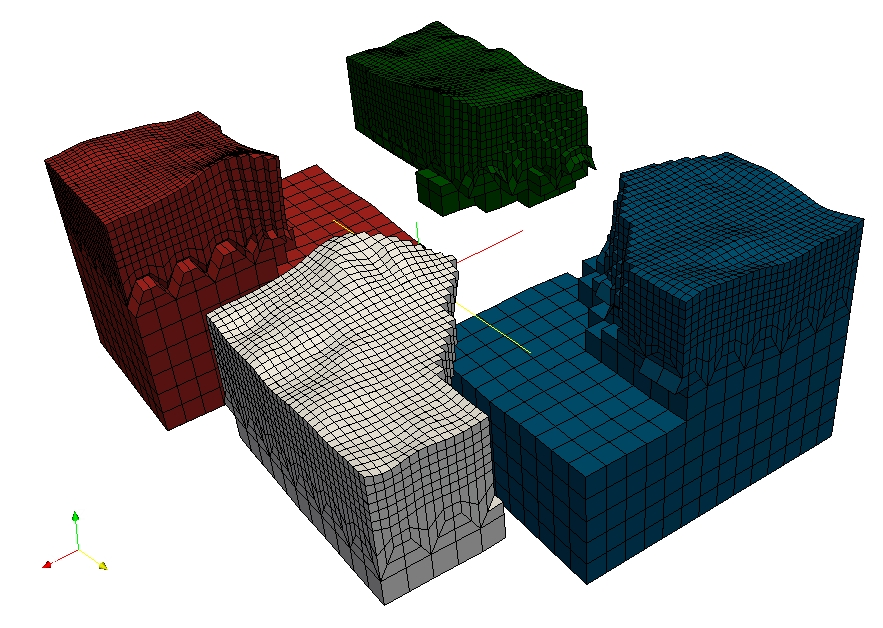
\includegraphics[width=0.45\textwidth]{figures/mount-partitions2.jpg}
\par
\end{centering}
\caption{Example of a mesh partitioning onto four cores. Each single core partition
is colored differently. The executable \texttt{xdecompose\_mesh} can
equally distribute the mesh on any arbitrary number of cores. Domain
decomposition is explained in detail in \citet{MaKoBlLe08}, and excellent
scaling up to 150,000 processor cores in shown for instance in
\citet{CaKoLaTiMiLeSnTr08,KoLaMi08a,MaKoBlLe08,KoErGoMi10,Kom11}.}
\label{fig:mount.partitions}
\end{figure}


When you are ready to compile, in the main directory type
{\small
\begin{verbatim}
make xdecompose_mesh
\end{verbatim}
}
\noindent
If all paths and flags have been set correctly, the executable \texttt{bin/xdecompose\_mesh}
should be produced.

The partitioning is done in serial for now (in the next release we
will provide a parallel version of that code). It needs to be run in the main directory because it expects the \texttt{./DATA/Par\_file}.
The synopsis is:
%
\begin{verbatim}
./bin/xdecompose_mesh nparts input_directory output_directory
\end{verbatim}
%
\noindent
where
\begin{itemize}
\item \texttt{nparts} is the number of partitions, i.e., the number of cores
for the parallel simulations,
\item \texttt{input\_directory} is the directory which holds all the files
generated by the Python script \texttt{cubit2specfem3d.py} explained
in the previous Section~\ref{subsec:Exporting-the-Mesh}, e.g. \texttt{./MESH/},
and
\item \texttt{output\_directory} is the directory for the output of this
partitioner which stores ACII-format files named like \texttt{proc{*}{*}{*}{*}{*}{*}\_Database}
for each partition. These files will be needed for creating the distributed
databases, and have to reside in the directory \texttt{LOCAL\_PATH}
specified in the main \texttt{Par\_file}, e.g. in directory \texttt{./OUTPUT\_FILES/DATABASES\_MPI}.
Please see Chapter~\ref{cha:Creating-Distributed-Databases} for
further details.
\end{itemize}
Note that all the files generated by the Python script \texttt{cubit2specfem3d.py}
must be placed in the \texttt{input\_directory} folder before running
the program.


\section{Meshing with \texttt{xmeshfem3D}}\label{cha:Running-the-Mesher-Meshfem3D}

In case you successfully ran the configuration script, you are also
ready to compile the internal mesher. This is an alternative to CUBIT
for the mesh generation of relatively simple models.
%
\begin{figure}[htbp]
\begin{centering}
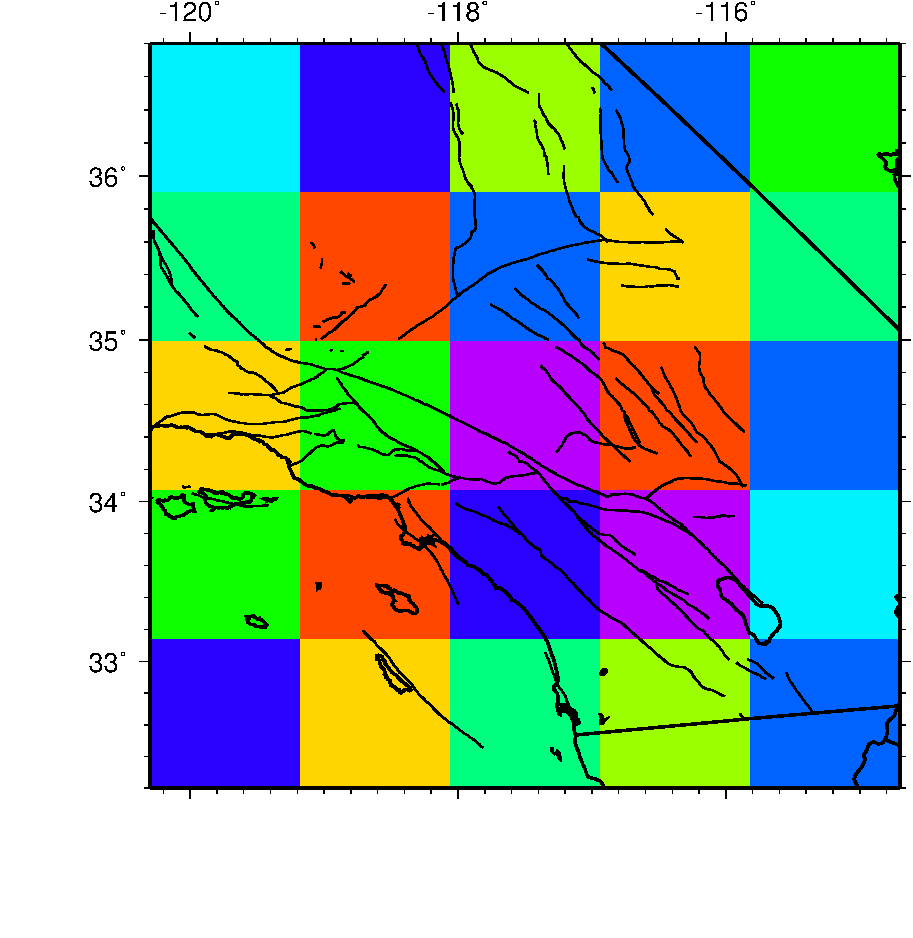
\includegraphics[scale=0.5]{figures/socal_map_mpi.pdf}
\par
\end{centering}
\caption{For parallel computing purposes,
the model block is subdivided in $\nprocxi\times\nproceta$ slices
of elements. In this example we use $5^{2}=25$ processors. }
\label{fig:For-parallel-computing}
\end{figure}


\noindent
In the main directory, type
{\small
\begin{verbatim}
make xmeshfem3D
\end{verbatim}
}
\noindent
If all paths and flags have been set correctly, the mesher should
now compile and produce the executable \texttt{bin/xmeshfem3D}. Please
note that \texttt{xmeshfem3D} must be called directly from the main
directory, as most of the binaries of the package.

Input for the mesh generation program is provided through the parameter
file \texttt{Mesh\_Par\_file}, which resides in the subdirectory \texttt{DATA/meshfem3D\_files/}.
(to see how to use it, see the EXAMPLES specific to the internal mesher in directory \texttt{EXAMPLES/meshfem3D\_examples/}.
Before running the mesher, a number of parameters need to be set in
the \texttt{Mesh\_Par\_file}. This requires a basic understanding
of how the SEM is implemented, and we encourage you to read \citet{KoVi98,KoTr99}
and \citet{KoLiTrSuStSh04}.

The mesher and the solver use UTM coordinates internally, therefore
you need to define the zone number for the UTM projection (e.g., zone
11 for Los Angeles). Use decimal values for latitude and longitude
(no minutes/seconds). These values are approximate; the mesher will
round them off to define a square mesh in UTM coordinates. When running
benchmarks on rectangular models, turn the UTM projection off by using
the flag \texttt{\small SUPPRESS\_UTM\_PROJECTION},
in which case all `longitude' parameters simply refer to the $x$~axis, and
all `latitude' parameters simply refer to the $y$~axis. To run the
mesher for a global simulation, the following parameters need to be
set in the \texttt{\small Mesh\_Par\_file}:
%
\begin{description}
\item [{\texttt{LATITUDE\_MIN}}] Minimum latitude in the block (negative
for South).
\item [{\texttt{LATITUDE\_MAX}}] Maximum latitude in the block.
\item [{\texttt{LONGITUDE\_MIN}}] Minimum longitude in the block (negative
for West).
\item [{\texttt{LONGITUDE\_MAX}}] Maximum longitude in the block.
\item [{\texttt{DEPTH\_BLOCK\_KM}}] Depth of bottom of mesh in kilometers.
\item [{\texttt{UTM\_PROJECTION\_ZONE}}] UTM projection zone in
which your model resides, only valid when
\texttt{SUPPRESS\_UTM\_PROJECTION} is \texttt{.false.}.
Use a negative zone number for the Southern hemisphere:
the Northern hemisphere corresponds to zones +1 to +60,
the Southern hemisphere to zones -1 to -60.


We use the WGS84 (World Geodetic System 1984) reference ellipsoid for the UTM projection. If you prefer to use the Clarke 1866 ellipsoid,
edit file \texttt{src/shared/utm\_geo.f90}, uncomment that ellipsoid and recompile the code.

From \url{http://en.wikipedia.org/wiki/Universal_Transverse_Mercator_coordinate_system}:\\
The Universal Transverse Mercator coordinate system was developed by the United States Army Corps of Engineers in the 1940s.
The system was based on an ellipsoidal model of Earth. For areas within the contiguous United States
the Clarke Ellipsoid of 1866 was used. For the remaining areas of Earth, including Hawaii, the International Ellipsoid was used.
The WGS84 ellipsoid is now generally used to model the Earth in the UTM coordinate system,
which means that current UTM northing at a given point can be 200+ meters different from the old one.
For different geographic regions, other datum systems (e.g.: ED50, NAD83) can be used.

\item [{\texttt{SUPPRESS\_UTM\_PROJECTION}}] set to be \texttt{.false.}
when your model range is specified in geographical coordinates, and
needs to be \texttt{.true.} when your model is specified in Cartesian
coordinates. \noun{UTM projection zone in which your simulation region
resides.}
%
\item [{\texttt{INTERFACES\_FILE }}] File which contains the description
of the topography and of the interfaces between the different layers
of the model, if any. The number of spectral elements in the vertical
direction within each layer is also defined in this file.
%
\item [{\texttt{NEX\_XI}}] The number of spectral elements along one side of the
block. This number \textit{must} be 8~$\times$~a multiple of $\nprocxi$
defined below. Based upon benchmarks against semi-analytical discrete
wavenumber synthetic seismograms \citep{KoLiTrSuStSh04}, determined
that a $\nexxi=288$ run is accurate to a shortest period of roughly
2~s. Therefore, since accuracy is determined by the number of grid
points per shortest wavelength, for any particular value of $\nexxi$
the simulation will be accurate to a shortest period determined by
\begin{equation}
\mbox{shortest period (s)}=(288/\nexxi)\times2.\label{eq:shortest_period}
\end{equation}
 The number of grid points in each orthogonal direction of the reference
element, i.e., the number of Gauss-Lobatto-Legendre points, is determined
by \texttt{NGLLX} in the \texttt{constants.h} file. We generally use
$\mbox{\texttt{NGLLX\/}}=5$, for a total of $5^{3}=125$ points per
elements. We suggest not to change this value.
%
\item [{\texttt{NEX\_ETA}}] The number of spectral elements along the other side
of the block. This number \textit{must} be 8~$\times$~a multiple
of $\nproceta$ defined below.
%
\item [{\texttt{NPROC\_XI}}] The number of processors or slices along one side
of the block (see Figure~\ref{fig:For-parallel-computing}); we must
have $\nexxi=8\times c\times\nprocxi$, where $c\ge1$ is a positive
integer.
%
\item [{\texttt{NPROC\_ETA}}] The number of processors or slices along the other
side of the block; we must have $\nexeta=8\times c\times\nproceta$,
where $c\ge1$ is a positive integer.
%
\item [{\texttt{USE\_REGULAR\_MESH}}] set to be \texttt{.true.} if you
want a perfectly regular mesh or \texttt{.false.} if you want to add
doubling horizontal layers to coarsen the mesh. In this case, you
also need to provide additional information by setting up the next
three parameters.
%
\item [{\texttt{NDOUBLINGS}}] The number of horizontal doubling layers.
Must be set at least to \texttt{1} if \texttt{USE\_REGULAR\_MESH} is set to \texttt{.true.}.
Multiple mesh doublings can be chosen, for which each an \texttt{NZ\_DOUBLING\_**} entry must be given.
By default, we only provide two possible entries in the \texttt{Mesh\_Par\_file}.
For higher numbers of doubling layers, additional entries must be added.
\item [{\texttt{NZ\_DOUBLING\_1}}] The position of the first doubling layer
(only interpreted if \texttt{USE\_REGULAR\_MESH} is set to \texttt{.true.}).
\item [{\texttt{NZ\_DOUBLING\_2}}] The position of the second doubling
layer (only interpreted if \texttt{USE\_REGULAR\_MESH} is set to \texttt{.true.}
and if \texttt{NDOUBLINGS} is set to \texttt{2}). Doubling layers must be at least \texttt{2} layers apart.
The layer count starts from the bottom layer.
More entries must be listed by the user if \texttt{NDOUBLINGS} is larger than \texttt{2}.
\item [{\texttt{CREATE\_ABAQUS\_FILES}}] Set this flag to \texttt{.true.}
to save Abaqus FEA \urlwithparentheses{www.simulia.com} mesh files
for subsequent viewing. Turning the flag on generates files in the
\texttt{LOCAL\_PATH} directory. See Section~\ref{sec:Mesh-graphics}
for a discussion of mesh viewing features.
\item [{\texttt{CREATE\_DX\_FILES}}] Set this flag to \texttt{.true.} to
save OpenDX \urlwithparentheses{www.opendx.org} mesh files for subsequent
viewing.
\item [{\texttt{LOCAL\_PATH}}] Directory in which the partitions generated
by the mesher will be written. Generally one uses a directory on the
local disk of the compute nodes, although on some machines these partitions
are written on a parallel (global) file system (see also the earlier
discussion of the \texttt{LOCAL\_PATH\_IS\_ALSO\_GLOBAL} flag in Chapter~\ref{cha:Getting-Started}).

The mesher generates the necessary partitions in parallel, one set
for each of the $\nprocxi\times\nproceta$ slices that constitutes
the mesh (see Figure~\ref{fig:For-parallel-computing}). After the
mesher finishes, you can log in to one of the compute nodes and view
the contents of the \texttt{LOCAL\_PATH} directory to see the files
generated by the mesher. These files will be needed for creating the
distributed databases, and have to reside in the directory \texttt{LOCAL\_PATH}
specified in the main \texttt{Par\_file}, e.g. in directory \texttt{OUTPUT\_FILES/DATABASES\_MPI}.
Please see Chapter~\ref{cha:Creating-Distributed-Databases} for
further details.
%
\item [{\texttt{NMATERIALS}}] The number of different materials in your
model. In the following lines, each material needs to be defined as:

\begin{verbatim}
material_ID rho vp vs Q anisotropy_flag domain_ID
\end{verbatim}

\noindent
where
\begin{itemize}
\item \texttt{Q} : quality factor (0=no attenuation) for shear attenuation $Q_{\mu}$
\item \texttt{anisotropy\_flag} : 0=no anisotropy / 1,2,.. check with implementation
in \texttt{aniso\_model.f90}
\item \texttt{domain\_id} : 1=acoustic / 2=elastic
\end{itemize}
\item [{\texttt{NREGIONS}}] The number of regions in the mesh. In the following
lines, because the mesh is regular or 'almost regular', each region
is defined as:
\begin{verbatim}
NEX_XI_BEGIN NEX_XI_END NEX_ETA_BEGIN NEX_ETA_END NZ_BEGIN NZ_END material_ID
\end{verbatim}
\end{description}
%
The \texttt{INTERFACES\_FILE} parameter of \texttt{Mesh\_Par\_File}
defines the file which contains the settings of the topography grid
and of the interfaces grids. Topography is defined as a set of elevation
values on a regular 2D grid. It is also possible to define interfaces
between the layers of the model in the same way. The file needs to
define several parameters:
\begin{itemize}
\item The number of interfaces, including the topography. This needs to
be set at the first line. Then, from the bottom to the top of the
model, you need to define the grids with:
\item \texttt{SUPPRESS\_UTM\_PROJECTION} flag as described previously,
\item number of points along $x$ and $y$ direction (NXI and NETA),
\item minimal $x$ and $y$ coordinates (LONG\_MIN and LAT\_MIN),
\item spacing between points along $x$ and $y$ (SPACING\_XI and SPACING\_ETA)
and
\item the name of the file which contains the elevation values (in $y$.$x$
increasing order).
\end{itemize}
%
At the end of this file, you simply need to set the number of spectral
elements in the vertical direction for each layer. We provide a few
models in the {\texttt{EXAMPLES/}} directory.\\


Finally, depending on your system, you might need to provide a file
that tells MPI what compute nodes to use for the simulations. The
file must have a number of entries (one entry per line) at least equal
to the number of processors needed for the run. A sample file is provided
in the file \texttt{mymachines}. This file is not used by the mesher
or solver, but is required by the \texttt{go\_mesher} and \texttt{go\_solver}
default job submission scripts. See Chapter~\ref{cha:Scheduler}
for information about running the code on a system with a scheduler,
e.g., LSF.

Now that you have set the appropriate parameters in the \texttt{Mesh\_Par\_file}
and have compiled the mesher, you are ready to launch it! This is
most easily accomplished based upon the \texttt{go\_mesher} script.
When you run on a PC cluster, the script assumes that the nodes are
named n001, n002, etc. If this is not the case, change the \texttt{tr
-d `n'} line in the script. You may also need to edit the last command
at the end of the script that invokes the \texttt{mpirun} command.
See Chapter~\ref{cha:Scheduler} for information about running the
code on a system with a scheduler, e.g., LSF.

Mesher output is provided in the \texttt{OUTPUT\_FILES} directory
in \texttt{output\_mesher.txt}; this file provides lots of details
about the mesh that was generated. Please note that the mesher suggests
a time step \texttt{DT} to run the solver with. The mesher output
file also contains a table about the quality of the mesh to indicate
possible problems with the distortions of elements. Alternatively,
output can be directed to the screen instead by uncommenting a line
in \texttt{constants.h}:
\begin{verbatim}
! uncomment this to write messages to the screen
! integer, parameter :: IMAIN = ISTANDARD_OUTPUT
\end{verbatim}
To control the quality of the mesh, check the standard output (either
on the screen or in the \texttt{OUTPUT\_FILES} directory in \texttt{output\_mesher.txt})
and analyze the skewness histogram of mesh elements to make sure no
element has a skewness above approximately 0.75, otherwise the mesh
is of poor quality (and if even a single element has a skewness value
above 0.80, then you must definitely improve the mesh). To draw the
skewness histogram on the screen, type \texttt{gnuplot plot\_mesh\_quality\_histogram.gnu}.

